\section{Analyse}
<<<<<<< HEAD
\begin{figure}[h]
	\begin{center}
		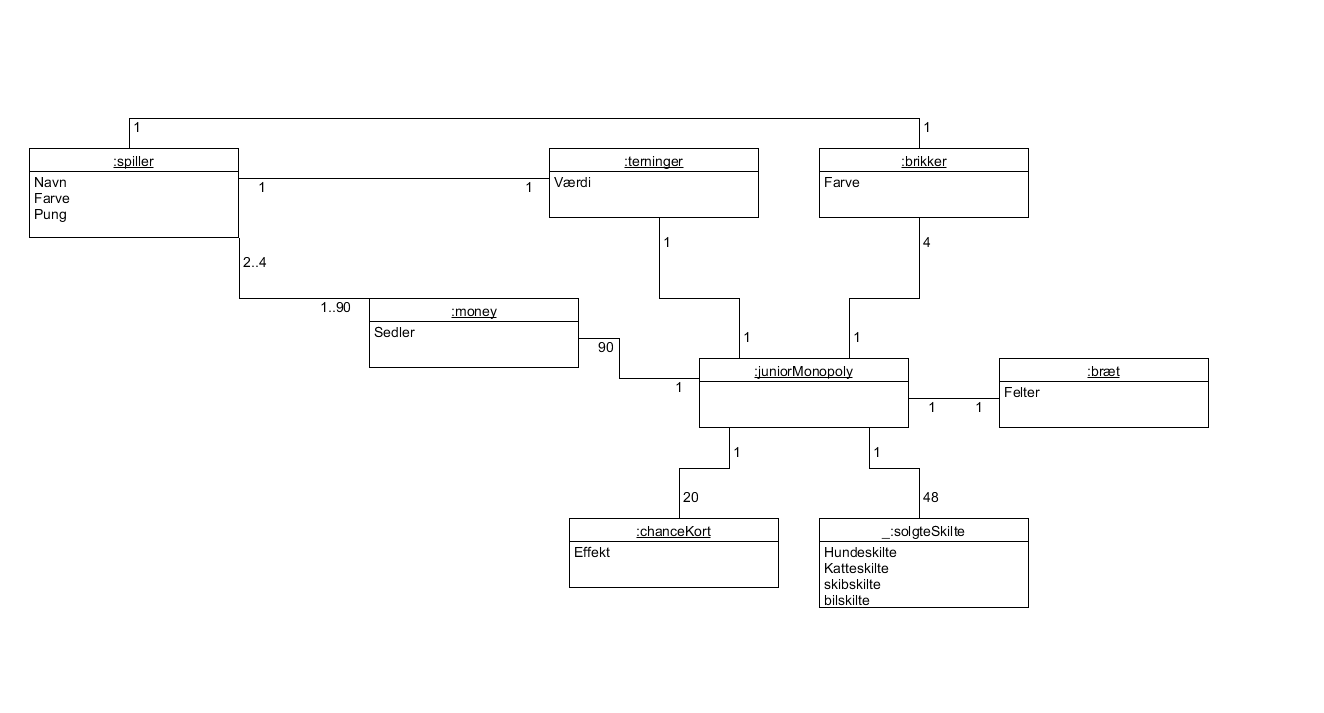
\includegraphics[scale=0.9]{fig/dtu/domainmodel.jpg}
	\end{center}
\end{figure}
	\subsection{UseCases}
=======
\subsection{Kravliste}
\begin{enumerate}
\item Spillet skal være mellem 2 - 4 personer
\item Spillerne skal slå terninger på skift
\item Der skal udskrives en tekst der omhandler det aktuelle felt, når spilleren lander på et felt
\item Hver felt skal have en effekt for spilleren
\item Spillerne starter med en balance på 30.000
\item Spillet slutter når alle undtagen en spiller er bankerot, altså når deres balance er nået 0
\item Spillerne skal kunne gå flere omgange rundt på spillepladen
\item Spillet skal kunne kører på DTU’s databarer
\end{enumerate}


\subsection{UseCases}
%1. UseCase
\begin{center}
    \begin{tabular}{ | m{10em} | m{10cm}| }
        \hline
            UseCase Section: Start af spil & Comment\\
        \hline
            Scope & Monopoly spil af IOOuterActive\\
        \hline
            Level & User-goal\\
        \hline
            Primær Aktør & IOOuterActive\\
        \hline
            Stakeholder og interessenter
            & IOOuterActive er interesseret i at spillerne skal kunne starte spillet\\
        \hline
            Forudsætninger & Spillet er installeret på enheden\\
        \hline
            Success guaranti & Spillet starter og spillerne bliver sendt videre til opsætning\\
        \hline
    \end{tabular}
\end{center}

%2. UseCase
\begin{center}
\begin{tabular}{ | m{10em} | m{10cm}| }
        \hline
            UseCase Section: Opsætning af spil & Comment\\
        \hline
            Scope & Monopoly spil af IOOuterActive\\
        \hline
            Level & User-goal\\
        \hline
            Primær Aktør & Spillerne\\
        \hline
            Stakeholder og interessenter & Spillerne er interesserede i at kunne vælge antal spillere og deres brikker\\
        \hline
            Forudsætninger & Spillet er startet op, og spillerne har nu mulighed for at vælge antal spillere og ønskede brikker\\
        \hline
            Success guaranti & Der er blevet valgt antallet af spillere, og hver spiller har valgt sin brik, herefter er spillet klar til at blive spillet\\
        \hline
    \end{tabular}
\end{center}
%3. UseCase
\pagebreak
Fully dressed UseCase:
\begin{center}
\begin{tabular}{ | m{10em} | m{10cm}| }
        \hline
            UseCase Section: Spillerne slår med terningerne & Comment\\
        \hline
            Scope & Monopoly spil af IOOuterActive\\
        \hline
            Level & User-goal\\
        \hline
            Primær Aktør & Spillerne\\
        \hline
            Stakeholder og interessenter & Spillerne er interesseret i at kunne trykke på en knap, og få et billede af to terninger med tilfældige værdier\\
        \hline
            Forudsætninger & Spillet er startet op, og spillerne har valgt antallet spillere og deres ønskede brikker\\
        \hline
            Success guaranti & Der er blevet valgt antallet af spillere, og hver spiller har valgt sit navn, herefter er spillet klar til at blive spillet\\
        \hline
            Hoved succes scenarie & Spillerne får udgivet en værdi af to terninger, og lander derefter på et felt\\
        \hline
            Alternative udfald & Negative udfald:\\
                & -	IOOuterActive har opdateret spillet, og derved opstår der en fejl når spillerne slå med terningerne, der kan ende i at der ikke bliver slået to terninger\\
                & -	Systemet blokerer for en spillers tur\\
                & -	En spiller hopper fra/på, og derved skal spillet startes om\\
        \hline
            Specielle krav
            & -	Enheden som spillet kører på skal være kompatibel med Java\\
            & -	Spillerne skal kunne interagere med GUI’en ved brug af mus eller touch\\
            & -	Der skal være plads på enheden til at kunne hente spillet\\
        \hline
            Hyppighed & Hver tur bliver der slået med terninger\\
        \hline
    \end{tabular}
\end{center}
%4. UseCase
\begin{center}
\begin{tabular}{ | m{10em} | m{10cm}| }
        \hline
            UseCase Section: Spiller køber et felt & Comment\\
        \hline
            Scope & Monopoly spil af IOOuterActive\\
        \hline
            Level & User-goal\\
        \hline
            Primær Aktør & Spillerne\\
        \hline
            Stakeholder og interessenter & Spillerne er interesseret i at købe det aktuelle felt\\
        \hline
            Forudsætninger & Spillet er i gang og en spiller har slået med terningerne\\
        \hline
            Success guaranti & Spilleren køber og ejer nu feltet\\
        \hline
    \end{tabular}
\end{center}

%5. UseCase
\begin{center}
\begin{tabular}{ | m{10em} | m{10cm}| }
        \hline
            UseCase Section: Spiller lander på et ejet felt & Comment\\
        \hline
            Scope & Monopoly spil af IOOuterActive\\
        \hline
            Level & User-goal\\
        \hline
            Primær Aktør & Spillerne\\
        \hline
            Stakeholder og interessenter & ****\\
        \hline
            Forudsætninger & Spillet er i gang og en spiller lander på et felt som er ejet af en anden spiller\\
        \hline
            Success guaranti & En spiller lander på et felt der er ejet af en anden spiller og får derfor en negativ effekt\\
        \hline
    \end{tabular}
\end{center}

%6. UseCase
\begin{center}
\begin{tabular}{ | m{10em} | m{10cm}| }
        \hline
            UseCase Section: En spiller taber & Comment\\
        \hline
            Scope & Monopoly spil af IOOuterActive\\
        \hline
            Level & User-goal\\
        \hline
            Primær Aktør & Terningerne\\
        \hline
            Stakeholder og interessenter & Spillerne er interesseret i at deres balance ikke når 0, og dermed taber\\
        \hline
            Forudsætninger & Spillerne har slået med terningerne\\
        \hline
            Success guaranti & En spiller lander på 0, og er ude af spillet\\
        \hline
    \end{tabular}
\end{center}

%7. UseCase
\begin{center}
\begin{tabular}{ | m{10em} | m{10cm}| }
        \hline
            UseCase Section: Spillet afsluttes & Comment\\
        \hline
            Scope & Monopoly spil af IOOuterActive\\
        \hline
            Level & User-goal\\
        \hline
            Primær Aktør & IOOuterActive\\
        \hline
            Stakeholder og interessenter & IOOuterActive er interesserede i at programmet viser en vinder og afsluttes\\
        \hline
            Forudsætninger & Alle spillere undtagen en, har fået en balance på 0\\
        \hline
            Success guaranti &Spillet viser en vinder og kan derefter afsluttes\\
        \hline
    \end{tabular}
\end{center}
\subsection{UseCase-Diagram}
    \begin{figure}[h]
        \advance\leftskip-3cm
        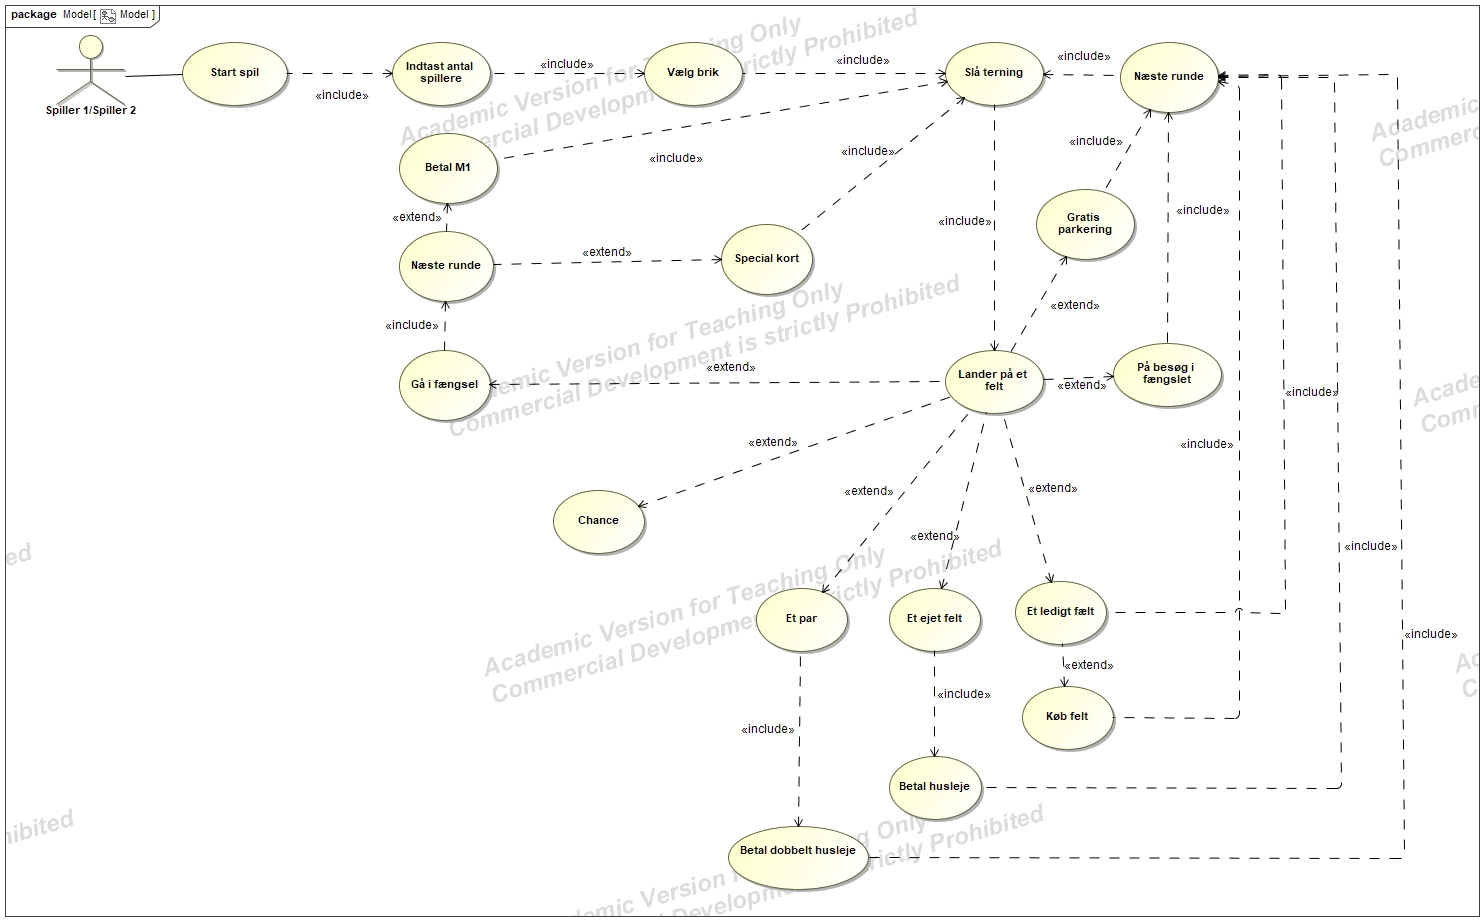
\includegraphics[width=20cm]{fig/UC-cdio3.jpg}
        \caption{Sekvensdiagram tegnet i MagicDraw}
    \end{figure}
\subsection{GRASP}
    GRASP står for General Responsibility Assignment Software Patterns. GRASP bruges til at give det rigtige ansvar til de forskellige klasser der bliver oprettet under udviklingen af et program. GRASP indeholder 9 patterns. Patterns bliver brugt til at strukturere et problem, samt at finde en passende løsning. De 9 patterns er:
    \begin{enumerate}
        \item Creator
        \item Information expert
        \item Low coupling
        \item Controller
        \item High cohesion
        \item Indirection
        \item Polymorphism
        \item Protected variations
        \item Pure fabrication
    \end{enumerate}
    (Der skrives mere når vi er nået længere i projektet)
>>>>>>> 1302cb58a29f8fab790c4f11e6a8c16de395ccb7
